%% A simple template for a lab or course report using the Hagenberg setup
%% with the standard LaTeX 'report' class
%% äöüÄÖÜß  <-- keine deutschen Umlaute hier? UTF-faehigen Editor verwenden!

\documentclass[a4paper,english,11pt]{report}
%\documentclass[a4paper,ngerman,11pt]{report}

\usepackage{hgb}
\usepackage{hgbabbrev}
\usepackage{hgblistings}
\usepackage{hgbbib}
\usepackage{hgbheadings}

\RequirePackage[utf8]{inputenc}		% remove when using lualatex oder xelatex!

\graphicspath{{images/}}  % where are the images?
\bibliography{literatur}  % requires file 'literatur.bib'

\author{Sascha Zarhuber\\ S1510629021}
\title{IM790 Thesis Project 2\\ \emph{Event-based build pipeline for static content management}\\ Project Report}
\date{\today}

%%%----------------------------------------------------------
\begin{document}
%%%----------------------------------------------------------
\maketitle
\tableofcontents
%%%----------------------------------------------------------

\chapter*{Abstract} % Vorwort

With a constantly growing number of internet users worldwide, websites are facing a difficult challenge nowadays: Serving information \emph{without delay}.

Static site generators build websites which don't need to interfere with any other service when requested by a client, and are therefore saving precious time and resources, if configured properly. A big drawback however is the amount of \emph{time}, \emph{configuration} and \emph{resources} needed for rebuilding the website every time its content changes.

This project should reveal possibilities to overcome these challenges, mainly by using a \emph{selective approach} to only render parts which have changed, but also by providing a REST API for outsourcing the build cycle to a remote service.


%%%----------------------------------------------------------
\chapter{Initial Situation}
%%%----------------------------------------------------------

Static site generators are growing fast and are more and more used as a replacement for common content management systems.

The main advantage are their independence of \emph{external} services, like database systems, session caching services, etc. Also, they seldomly consist of complicated backend systems and are mostly created in pure \emph{HTML} or simple markup languages like \emph{Markdown}\footnote{\url{https://daringfireball.net/projects/markdown/} -- Website of Markdown.}.
%
\begin{figure}[t]
    \centering
    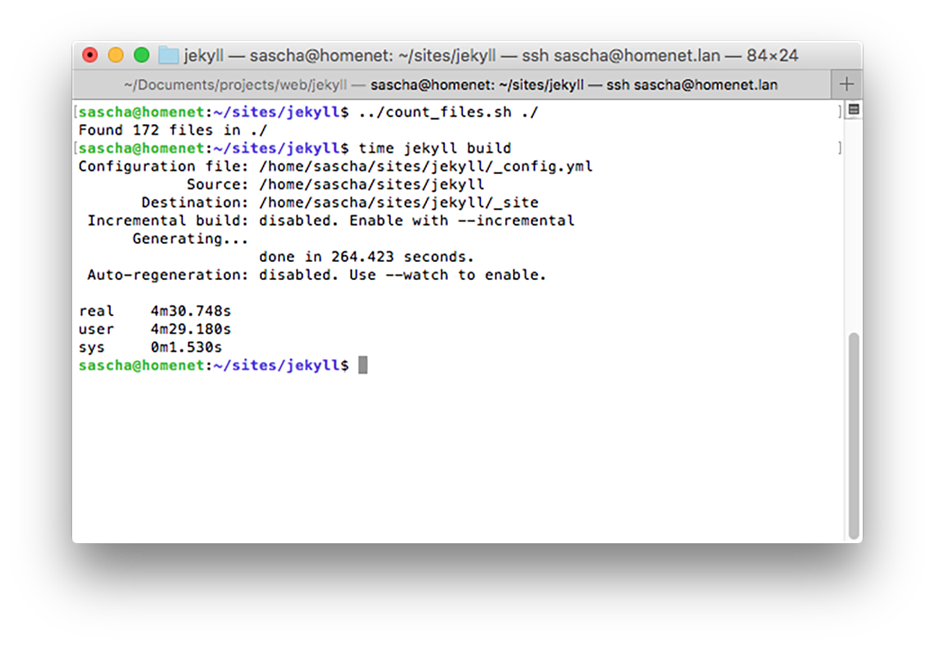
\includegraphics[width=0.8\textwidth]{jekyll_build.png}
    \caption{A screenshot showing the build time for the webroot of\newline \url{https://jekyllrb.com}. 172 files were generated in approximately 4:30 minutes. The result is a complete webroot containing browser readable HTML pages, assets, style sheets and JavaScript files.}
    \label{fig:jekyll_build}
\end{figure}
%

One of the biggest drawbacks however, is the fact, that static site generators have to preprocess every bit of information they contain (see Fig. \ref{fig:jekyll_build}). This is the complete opposite compared to other content management systems, which process information on request. This means, that user-readable content is fetched and rendered \emph{just in time} it was requested from the client.

Therefore, depending on the setup, a dynamically growing amount of time needed for a build cycle might be the case. For being able to work against this fact, a working approach has to be found, which saves time by \emph{leaving out} information, which has not changed since the previous build.

\section{Relation to Thesis Project 1}
\label{sec:relation-project}
This project is closely related to ``IM690 Thesis Project 1'', as the Thesis Project 1 was considered as intermediate result, whereas the current state of this project represents a usable version containing a static site generator wrapped in a REST API.

The status of Thesis Project 1 at submission included necessary REST API endpoints, together with a working configuration file parser and a file deletion possibility for slimming down the website sources prior instantiating the build pipeline. Furthermore, the authentication framework and the database connection were fully usable. The development steps for Thesis Project 2 concentrated on mainly refining the build services and making it as fail-safe as possible:

\begin{itemize}
  \item Restructured the build pipeline flow for enabling ``fail-early'' error handling.
  \item Improved the \emph{node modules} install service.
  \item Decoupled the build pipeline flow into an own child process to unblock the main event-loop.
  \item Enhanced the detection of previous builds by adding necessary information to build entries.
  \item Added compression (tar.gz) and distribution workflows at the end of the build cycle, enabled by events.
\end{itemize}

\section{Relation to written thesis}
\label{sec:relation-thesis}
The written thesis mainly shows different possibilites for improving build cycles of static site generators in theory, but concentrates on the considerations behind this project. Most importantly, it also evaluates this project in terms of usability and stability concerning high load on the REST API.

Because of the complexity of different parts used in this project, the thesis explains the state of the art, as well as the technical foundations necessary for development before any in-depth code documentation. Therefore, the reader should be able to follow the design decisions made in favor of the project outcome.

Lastly, a developer should get a good insight of how different web technologies, which may look contradictory at first sight, are able to interact seamlessly, although some sort of customization could be necessary.
%

%%%----------------------------------------------------------
\chapter{Implementation}
%%%----------------------------------------------------------

%
\begin{figure}[t]
    \centering
    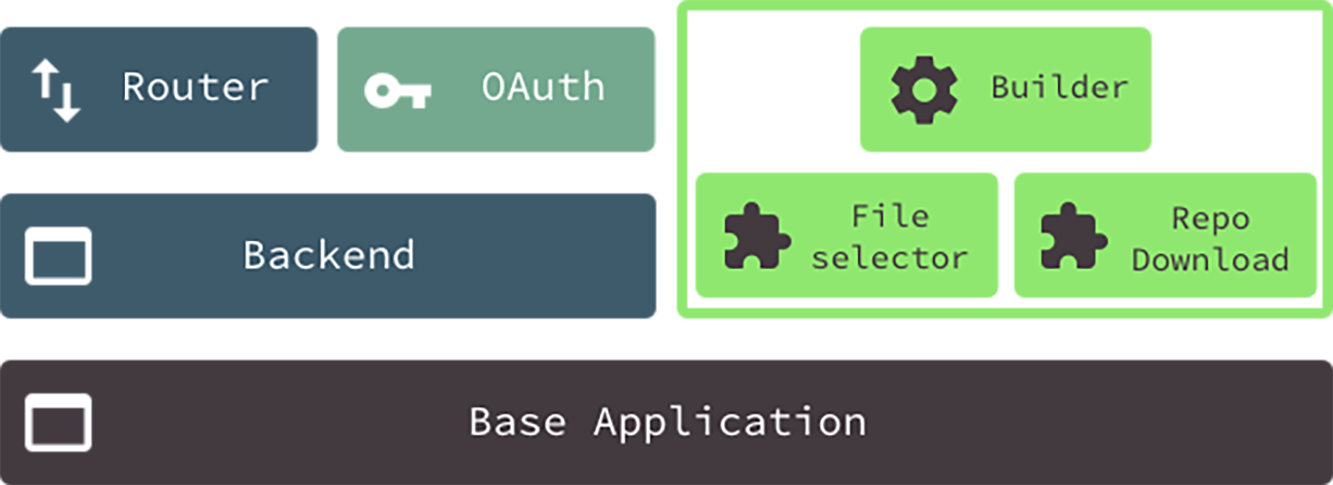
\includegraphics[width=0.9\textwidth]{application_structure.png}
    \caption{A graphic showing the base structure of the implemented application. The \emph{base application} layer serves as foundation, containing necessary libraries for implementing the \emph{HTTP} specifications. The \emph{routing} and \emph{OAuth} layer are responsible for authenticated requests to the endpoints, whilst the \emph{builder package} is designed as a partly autonomous, loosely coupled rendering service.}
    \label{fig:application_structure}
\end{figure}
%

The project itself was intended to work as a standalone service, thus leading to the advantage of not having to install a complete project setup locally on the content producer side. Additionally, one of the first design decisions was to closely couple this project with the \emph{GitHub API}\footnote{\url{https://developer.github.com/v3/} -- Documentation of GitHub API v3.}.

Both of these decisions should lead to a fully customizable production environment, easy to setup and adapted to each desired workflow, without having the need of making a compromise prior to getting workload done.

\section{Framework choice}
Although there are a lot of static site generator frameworks available, I mainly concentrated on comparing the following two, before setting up my project application:

\subsection{Jekyll}
\emph{Jekyll}\footnote{\url{https://jekyllrb.com} -- Website of Jekyll.} -- the leading static site generator with more than 28,000 stars on GitHub\footnote{\url{https://github.com/jekyll/jekyll} -- Jekyll on GitHub.}, was responsible for a renaissance of statically generated websites, when it was introduced in 2008\footnote{\url{https://jekyllrb.com/docs/history/} -- History of Jekyll}.

Originally introduced by \emph{Tom Preston-Werner}, one of the co-founders of GitHub, it quickly grew a big community around it, benefitted mostly due to its wide usage on \emph{GitHub Pages}\footnote{\url{https://pages.github.com} -- GitHub's Pages service}. However, Jekyll is written in \emph{Ruby}, which causes a bit of friction, when trying to embed it into a server-side JavaScript-based ecosystem.

\subsection{Metalsmith}
\emph{Metalsmith}\footnote{\url{http://www.metalsmith.io} -- Website of Metalsmith.} -- a very modular static site generator on the other hand, is completely written in JavaScript, which makes it easier to integrate it into \emph{Node.js}-based applications. Furthermore, it consists basically just of modules, so that every job inside the build pipeline gets handled from its own module. The whole application may be put together and extended like using \emph{LEGO} bricks.

Due to the possibility of heavily customizing a Metalsmith setup to your needs, the decision was made in favor of this framework, although a few challenges remained:

\begin{itemize}
  \item A working remap of Jekyll's variable structure to Metalsmith could not be realized. Both projects handle their build cycles too different. This makes it even harder to compare my intended selective approach to conventional Jekyll project setups.
  \item Shopify's Liquid template engine has not been fully ported to JavaScript till this day. It easily breaks when using custom functionality within template files.
  \item Custom project setups in general require a customized, adaptive handling during build time. This concerns not only Jekyll projects, but also customized Metalsmith projects.
\end{itemize}

\section{Application structure}
The application itself was bootstrapped from an \emph{Express.js}\footnote{\url{https://expressjs.com} -- Website of Express.js.} base configuration. To persist user, project and build information, the online \emph{MongoDB}-service \emph{mLab}\footnote{\url{https://mlab.com} -- Website of mLab.} was used, as it provides a free tier for testing purposes.

Using this persistence possibility, an additional authentication service was realized using \emph{OAuth2orize}\footnote{\url{https://github.com/jaredhanson/oauth2orize} -- OAuth2orize repository on GitHub.}. This makes it easier to provide an application-wide user management system, which does not require any HTML login form.

At the end of last semester, the application featured a routing service to different API endpoints, an \emph{OAuth2.0} authentication service and a decoupled building service containing access to the GitHub API, as well as a very basic \emph{Metalsmith} setup (see Fig. \ref{fig:application_structure}).

The Metalsmith setup was since enhanced, as well as the decoupled build pipeline. Both are outsourced into an own child process now, leaving the REST API as reliable and responsive as initially intended -- the communication channel between parent and child process cares for optimal information exchange.

\subsection{Challenges}
After providing a basic working example in the last semester, a few major challenges had to be solved during the ongoing development. These challenges were mostly caused by diving deeper into Node.js' low-level environment without any prior experience.

The probably most significant impact in any further development was the introduction of child process handling during a build cycle. Due to Node.js' asynchronous and event-driven ecosystem, any blocking operations are possibly causing major delay and may lead to an unresponsive web application. By forking a child process, it is possible to keep the event loop responsive while executing a blocking task on a separate process.

Thus, concurrent build cycles of different projects are possible, as every rendering process is being outsourced and managed via events from the main process. The executing user receives an intermediate result with a reference to a database entry for further information about the status of the current build operation.

Other challenges were mostly caused by the general interaction with the GitHub API, as well as the time management behind asynchronous requests and their subsequent evaluation.

\subsection{Implemented request flow}
The finished REST API now consists of a fully working request flow, which was being optimized for speed and reliability. Whether a build cycle succeeded or failed, the client receives a response using the ``fail-early'' principle~--~this means, that the most error-prone tasks are processed in an early stage of the build process. These possibly error-prone tasks contain the following:

\begin{itemize}
  \item examination of the file tree and retrieving various file paths,
  \item fetching and parsing of the configuration file,
  \item fetching the latest build entry and comparing the commit hash, as well as
  \item requesting the commit range and filtering the affected files.
\end{itemize}
After completion of the above tasks, a new build log is stored in the database and the client receives a response with the current, intermediate data. Then, the child process is forked, and the heaviest task of the build pipeline is initiated: creating and configuring the Metalsmith instance.

After everything went well, the database entry is updated accordingly and the finished outcome of the rendering task is compressed as tar.gz-archive for deployment on any desired web server (see Figs. \ref{fig:request_flow} and \ref{fig:application_flow}).

%
\begin{figure}
    \centering
    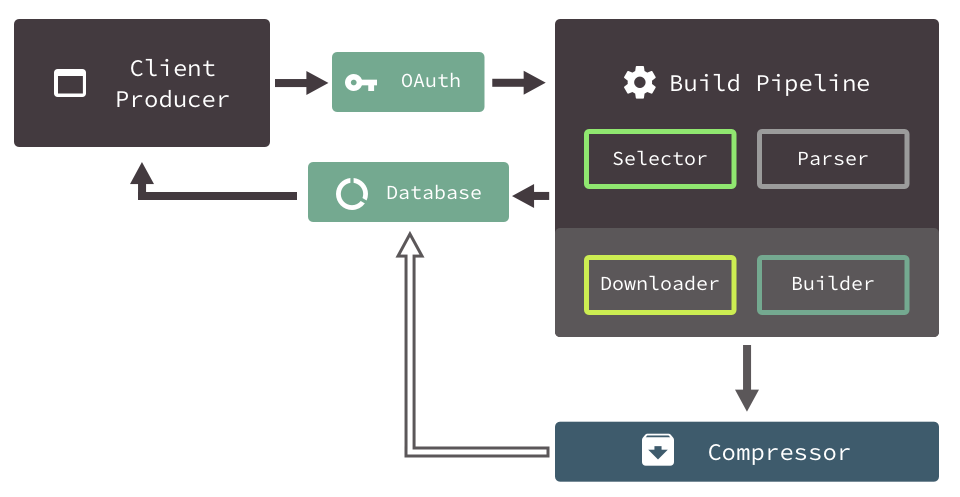
\includegraphics[width=0.9\textwidth]{request_flow.png}
    \caption{A graphic showing the request flow of the REST API. The \emph{client producer} requests the build endpoint on the REST API; the \emph{OAuth} layer first authorizes the request by verifying the access token in the request header, then the request is handled by the \emph{build pipeline}. The build pipeline consists of a collection of tasks which are grouped and either handled concurrently or sequentially. Before forking the child process (light brown background), the intermediate status is written to the \emph{database} and returned to the client producer. Afterwards, the outcome is compressed to a \emph{tar.gz}-archive and the database entry is updated accordingly.}
    \label{fig:request_flow}
\end{figure}
%

%
\begin{figure}
    \centering
    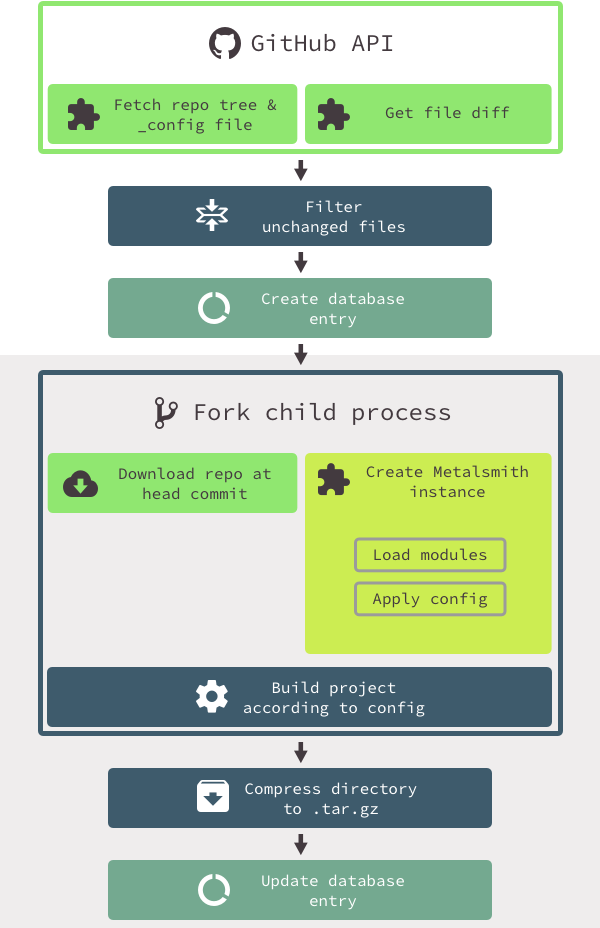
\includegraphics[width=0.9\textwidth]{application_flow.png}
    \caption{A graphic showing the main application flow of the build pipeline from top to bottom. At first, the \emph{repo tree} and \emph{file diff} are fetched from the GitHub API in parallel. After file filtering and creating a database entry, a child process is forked, which cares for executing the heavy tasks for building. After a successful build, the resulting files are compressed into a \emph{tar.gz} archive, then the database entry is updated accordingly. Afterwards, the child process is terminating gracefully.}
    \label{fig:application_flow}
\end{figure}
%

\section{Selective approach}
To get a basic overview on which parts have changed, a file comparison using \emph{diff} is very supportive in this case. Not only does it show how different files have been altered (\emph{added}, \emph{modified} or \emph{deleted}), but also which contents faced a change.

Luckily, the GitHub API already provides certain diff information using a \emph{JSON}-formatted structure\footnote{\url{https://developer.github.com/v3/repos/commits/\#compare-two-commits} -- ``Compare two commits'' documentation on GitHub.}.
Parsing a diff file is therefore not necessary anymore, as the GitHub API returns this sort of information based on the \emph{base} and \emph{head} commit hash present as request parameters.

The only thing left is to filter out every file path from the object and decide whether it is a content file or a system file. If there were only content files present in the commit comparison, only these have to be built, as all the other content files are already rendered and available. At the end of the build process the rendered content files only need to be merged with the existing, previous file tree to form an updated version of the website.

\section{Summary}
\label{sec:summary}
As a summary it can be said, that although this is a working web application, it has to be seen as proof of concept in the first place. The reason is simple: as the REST API needs different access tokens and keys to work with the various online services, it can not be easily customized to a multi-user environment at the moment.

The experience I gained from working on a project of such a size on the other hand was very important, since I hardly ever worked on such a low level in JavaScript. Therefore the most important lessons I've learned during the last semester are:

\begin{itemize}
  \item Find the correct balance of responsiveness and functionality, outsource heavy, blocking tasks to child processes if possible, but care for a clean communication and data exchange between parent and child.
  \item Include automated tests into the development workflow as soon as possible, many small refactorings concerning the correct distribution of sub-tasks (config parsing, repository downloading, etc.) could have been avoided in the first place.
  \item Have an online testbed available, as online services are likely to behave differently than a local workstation.
\end{itemize}
Looking back, using Node.js was the right choice for this project, as especially its modular and enhanceable features supported me in a way, that an ongoing development was possible and even bigger changes did not cause a major rework on dependent parts of the application.

Metalsmith also played an important part, as its extensible plugin handling supported me in filling the gap between heavily customized projects and the build pipeline's interface to the REST API. Together with Express.js as well-tested REST framework, it now features a semi-automatic build pipeline, which is responsive to HTTP requests.

\subsection{Future development}
Future development would definitely have to include a graphical user interface in the browser, as pure CLI and HTTP request based operations are error-prone and confusing at some point. Especially build errors would be easier to display and visualize.

Furthermore, a graphical user interface would also offer the possibility of opening the project to multiple users by supporting a correct authorization flow between the REST API and GitHub. Currently authorization is done by storing a certain access token into an environment variable, leading to a very limited support of repositories on GitHub.

%%%----------------------------------------------------------
\chapter{Milestones acquired}
%%%----------------------------------------------------------

\begin{itemize}
\item Rework requests to GitHub API
\item Provide ecosystem for web project builds
\item Select files using GitHub's commit comparison
\item Keep track on build states
\item Refactor testbed for render measurements
\end{itemize}



%%%----------------------------------------------------------
\chapter{Intended project goals}
%%%----------------------------------------------------------

\begin{itemize}
\item Render or re-render static webroots seamlessly
\item Provide latest build as archive for deployment
\item Make service responsive to GitHub webhooks
\item Integrate into CI services
\end{itemize}


%%%----------------------------------------------------------
%\MakeBibliography[nosplit]
%%%----------------------------------------------------------

\end{document}
